\hl{L5:GNN2}
\hlgreen{graph convolution}
\hlorange{Laplacian matrix} For a given graph \( g = (V, E) \) with \( A \) as its adjacency matrix, its Laplacian matrix is defined as \( L = D - A, \) where \( D \) is a diagonal degree matrix \( \text{diag}(d_{v1}, \dots, d_{v_2}) \) 
% \textcolor{red}{Eigen-decomposition of Laplacian Matrix}
Laplacian matrix is a difference operator:
\( h = Lf = (D - A)f = Df - Af \quad (f \in \mathbb{R}^{n \times 1}) \)
\( h(i) = \sum_{ v_j \in N(v_i)}(f(i) - f(j)) \quad  \)
Laplacian quadratic form: \( f^T L f = \frac{1}{2} \sum_{i,j=1}^{N} A[i,j](f(i) - f(j))^2 \)
\hlorange{Spectral-Based Graph Convolution}  First apply Graph Fourier Transform (GFT) on the graph to obtain its Graph Fourier coefficients, and then modulate these coefficients before reconstructing the signal in the spatial domain. the graph filters can be learned.
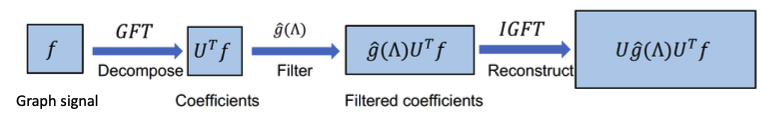
\includegraphics[height=0.02\textwidth]{figs/l5-1.png}
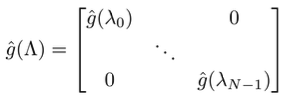
\includegraphics[height=0.018\textwidth]{figs/l5-2.png}
\hlorange{limitations of Primal Graph Filter:} 1. \# of learned parameters is equal to \# of nodes N; 2. convolution operator is not spatially localized; 3. eigen decomposition of the Laplacian matrix is computational expensive.
\hlorange{Polynomial Filter Operator}Spectral Decomposition:
\(
\mathbf{L} = \mathbf{U} \mathbf{\Lambda} \mathbf{U}^T
\)
k-order Polynomial Filter Operator:
\(
g(\mathbf{\Lambda}) = \sum_{k=0}^{K} \theta_k \mathbf{\Lambda}^k
\), 
\(f'= \mathbf{U} g(\mathbf{\Lambda}) \mathbf{U}^T \mathbf{f}
= \sum_{k=0}^{K} \theta_k \mathbf{U} \mathbf{\Lambda}^k\mathbf{U}^T f=\sum \theta_kL^kf
\), 
\(\mathbf{U} \mathbf{\Lambda}^k\mathbf{U}^T = \mathbf{U} (\mathbf{\Lambda}\mathbf{U}^T\mathbf{U})^k\mathbf{U}^T = L^k\)
\hlorange{Limitations of Polynomial Filter} $g(x)=\theta_0 + \theta_1x+\theta_2x^2$ 1. Non-orthogonal; 2. Unstable under perturbation of coefficients
\hlorange{Chebyshev Polynomials} form an orthogonal basis for the Hilbert space
\(
T_0(x) = 1;
T_1(x) = x;
T_k(x)= 2xT_{k-1}( x) - T_{k-2}(x);
g (x) = \theta_0 T_0( x) + \theta_1 T_1( x) + \theta_2 T_2 (x) + \cdots
\), 
\(
\hat{g}(\mathbf{\Lambda}) = \sum_{k=0}^{K} \theta_k T_k(\Tilde{\mathbf{\Lambda}}), \Tilde{\mathbf{\Lambda}}=\frac{2\Lambda}{\lambda_{max}}-1
\),
\(f'= \mathbf{U} \hat{g}(\mathbf{\Lambda}) \mathbf{U}^T \mathbf{f} = \sum_{k=0}^{K} \theta_k T_k(\Tilde{\mathbf{\Tilde{L}}})f, \Tilde{L} =  \frac{2L}{\lambda_{max}}-1\)
\hlorange{GCN: simplified chebNet} K = 1 and $\lambda_{max}=2, \theta=\theta_0=-\theta_1$, \(\hat{g}(\mathbf{\Lambda})=\theta_0 + \theta_1(\Lambda-I) = \theta(2I-\Lambda, \mathbf{U} \hat{g}(\mathbf{\Lambda}) \mathbf{U}^T \mathbf{f}=\theta(2I-L)f=\theta\left(\Tilde{D}^{-\frac{1}{2}}A D^{-\frac{1}{2}} \right)f, \Tilde{A} = A+I \)
\hlorange{Spatial-Based Graph Convolution} \(H^{(l+1)} = \sigma\left(D^{-\frac{1}{2}}A D^{-\frac{1}{2}} H^{(l)} W^{(l)}\right)\) 
spatial-based GNNs including GCN, GraphSAGE and GAT are special cases of Message PassingNN
\hlorange{GraphSAGE} Aggregate: mean, lstm, pool; here is the mean form: \(h_{v}^{(k)} = \sigma\left( W \cdot \text{CONCAT}\left( h_{v}^{(k-1)}, \frac{1}{|\mathcal{N}(v)|} \sum_{u \in \mathcal{N}(v)} h_{u}^{(k-1)} \right) \right)\) $h_{v}^{(k)}$ is the feature representation of node $v$ at the $k^{th}$ layer. $\mathcal{N}(v)$ denotes the set of neighbors of node $v$.
\hlorange{attention} 1. The attention score between a query $q$ and a key $k_i$ is:
\(
\text{score}(q, k_i) = q \cdot k_i^T
\)
2. The attention weights are computed using a softmax over the scores:
\(
\alpha_i = \frac{\exp(\text{score}(q, k_i))}{\sum_{j=1}^{T}\exp(\text{score}(q, k_j))}
\)
3. The attention output is a weighted sum of the values:
\(
\text{Attention output} = \sum_{i=1}^{T} \alpha_i v_i
\)
\hlorange{GAT} The Graph Attention Network (GAT) updates node features based on the following:
% \textcolor{red}{GCN, ChebNet, GAT, GraphSAGE}
1. Compute the attention coefficients between nodes $v$ and $u$:
\(
e_{vu} = \text{LeakyReLU}\left(\mathbf{a}^T [\mathbf{W} \mathbf{h}_v \parallel \mathbf{W} \mathbf{h}_u] \right)
\)
2. Normalize the attention coefficients with softmax:
\(
\alpha_{vu} = \frac{\exp(e_{vu})}{\sum_{k \in \mathcal{N}(v)} \exp(e_{vk})}
\)
3. Update the node features using the normalized attention weights:
\(
h_v' = \sigma \left( \sum_{u \in \mathcal{N}(v)} \alpha_{vu} \mathbf{W} \mathbf{h}_u \right)
\)
where $\mathcal{N}(v)$ denotes the neighbors of node $v$, and $\sigma$ is an activation function.
\hlgreen{Graph Pooling}Flat Graph Pooling and Hierarchical Graph Pooling. 
\hlorange{Flat Graph Pooling } 1. The max-pooling and average pooling operations in classical CNNs can be directly adopted to GNNs. 2. Attention-Based Flat Pooling 1. Compute an attention score for each node:
\(
s_i = \mathbf{a}^T \tanh(\mathbf{W} \mathbf{h}_i)
\)
2. Normalize the scores with softmax:
\(
\alpha_i = \frac{\exp(s_i)}{\sum_{j=1}^{N} \exp(s_j)}
\)
3. Compute the graph representation using the attention weights:
\(
\mathbf{h}_{\text{graph}} = \sum_{i=1}^{N} \alpha_i \mathbf{h}_i
\)
\hlorange{Hierarchical Graph Pooling}  Flat graph pooling ignores the hierarchical sub-graph structure information; Hierarchical graph pooling layers aim to preserve the hierarchical graph structural information by coarsening the graph step by step. 
\hlorange{Downsampling-Based Graph Pooling: gpool}
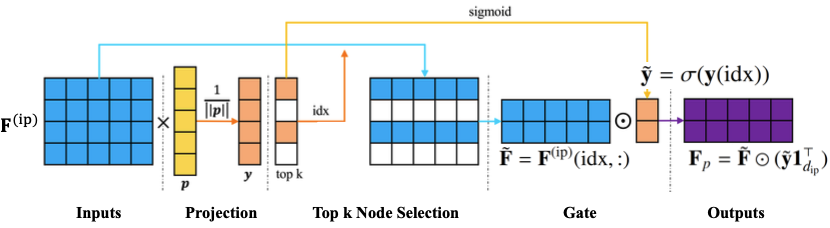
\includegraphics[height=0.022\textwidth]{figs/l5-4.png} 
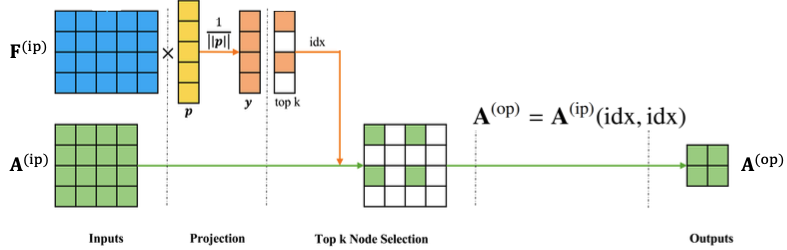
\includegraphics[height=0.022\textwidth]{figs/l5-3.png} 
% \textcolor{red}{Page 65 gPool and DiffPool}
\hlorange{Supernode-Based Graph Pooling: diffpool}
\(S = \text{softmax}(\text{GCN}(A^{ip}, F^{ip}) \in \mathbb{R}^{N_{ip} \times N_{op}}), A^{op}=S^TA^{ip}, F^{op}=S^TGCN(A,F)
\)
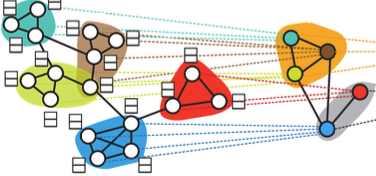
\includegraphics[height=0.022\textwidth]{figs/l5-5.png} 
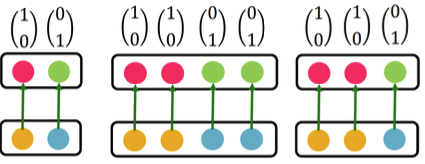
\includegraphics[height=0.022\textwidth]{figs/l6-8.png}
\hl{L6:GNN3} GCN and GraphSAGE’s aggregation functions fail to distinguish some basic multi-sets; hence not injective. GCN (mean-pool): 
$\text{Mean}({f_{u}} n \in N(v)) $
GraphSAGE(max-pool)$\text{Max}({f_{u}} n \in N(v)) $
Function \( g: X \rightarrow Y \) is injective if it maps different elements into different outputs.
\hlorange{Graph Isomorphism Network} 
% \textcolor{red}{formula Page 14 to 25} 
\hlorange{Comparison Between GIN and WL Graph Kernel} 1.Node embeddings are low-dimensional; hence, they can capture the fine-grained similarity of different nodes. 2.Parameters of the update function can be learned for the downstream tasks; 3. Because of the relation between GIN and the WL graph kernel, their expressive is exactly the same. If two graphs can be distinguished by GIN, they can be also distinguished by the WL kernel, and vice versa. 4. \textcolor{blue}{GIN is also powerful enough to distinguish most of the real graphs!}
\hlorange{Improving Expressive Power}GIN and MPNN cannot distinguish some basic graph structures like counting the cycle length. the computation graph for node A and B are same.
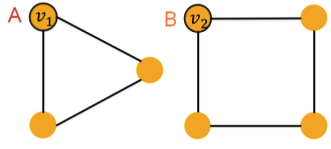
\includegraphics[height=0.02\textwidth]{figs/l6-1.png} 
\hlorange{Position-aware GNNs} 
\hlpurple{Anchors:} 1.Randomly pick node \( s1 \) and \( s2 \) as anchor nodes, which can be used to locate nodes in the graph.2. Represent \( v1 \) and \( v2 \) via their relative distances w.r.t. the anchors
\hlpurple{Anchor sets}1. Generalize anchor from a single node to a set of nodes. 2. We define distance to an anchor-set as the minimum distance to all the nodes in the anchor-set 3. Large anchor-sets provide better position estimation.
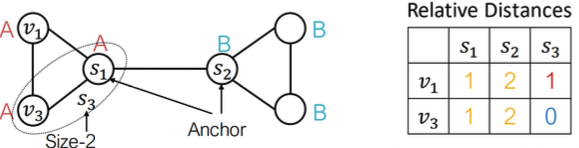
\includegraphics[height=0.03\textwidth]{figs/l6-2.png} How to use position encoding? The simple way: use position encoding as augmented node features (works well in practice). 
\hlpurple{Issue}: if we permute the dimensions of position encoding, the output will change.
\hlpurple{Solution} 1. Sample multiple anchor-sets \( S1 \), \( S2 \), and \( S3 \). 2. For node \( v1 \), aggregate information from anchor-sets \( S1 \), \( S2 \), \( S3 \) to obtain embeddings \( Mv1[1] \), \( Mv2[2] \), \( Mv3[3] \). 3. Aggregate \( Mv1[1] \), \( Mv2[2] \), \( Mv3[3] \) to obtain \( hv1 \) (for next layer) and position embedding \( zv1 \) (for output).
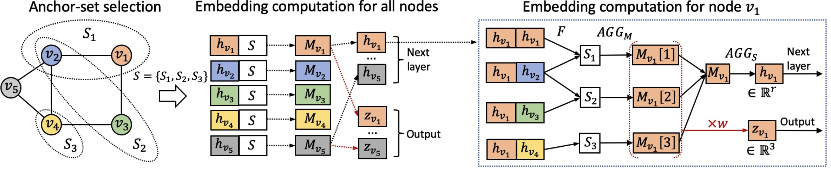
\includegraphics[height=0.035\textwidth]{figs/l6-3.png}
\hlorange{Identity-aware GNNs} Inductive node coloring can help distinguish specific graph structures: Different computational graphs -> successfully differentiate nodes.
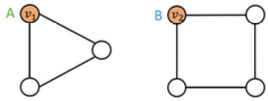
\includegraphics[height=0.025\textwidth]{figs/l6-4.png}
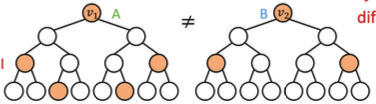
\includegraphics[height=0.025\textwidth]{figs/l6-5.png}
\hlorange{Heterogenous message passing} ID-GNN: at a given layer, different message/aggregation to nodes with different colorings.
\hlorange{Why heterogenous message passing works}1. Suppose two nodes have the same computational
graph, but have different node colorings. 2. Since we apply different neural network for computation, their embeddings will be different.
\hlorange{Summary} 1. ID-GNN is the first message passing framework that is more expressive than 1-WL test. 2. ID-GNN can count cycles originating from a given node, but GNN cannot. 3.ID-GNN can be applied to enhance any message passing GNNs (GCN, GraphSAGE, GIN, ...)
\hlorange{Over-smoothing in GNNs} Stack GNN layers sequentially, which can aggregate multi-hop neighboring nodes. When stacking K-layer GNN, each node has a receptive field of K-hop neighborhood.
\hlorange{Over-smoothing}: all the node embeddings converge to the same value. This is bad because we want to use node embeddings to differentiate nodes. \hlpurple{Reason: } The shared neighbors quickly grows when we increase \# hops (\# GNN layers). Embedding of a node is determined by its receptive field, if two nodes have highly-overlapped receptive fields, then their embeddings are highly similar.
\hlpurple{Solution: }Skip Connection, DropEdge, PairNorm.
\hlorange{Skip Connection} adding shortcuts in GNN. \( N \) skip connections \( \rightarrow \) \( 2^{N} \) possible paths. We automatically get a mixture of shallow GNNs and deep GNNs.
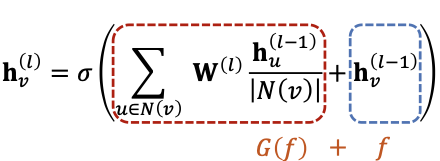
\includegraphics[height=0.025\textwidth]{figs/l6-6.png}
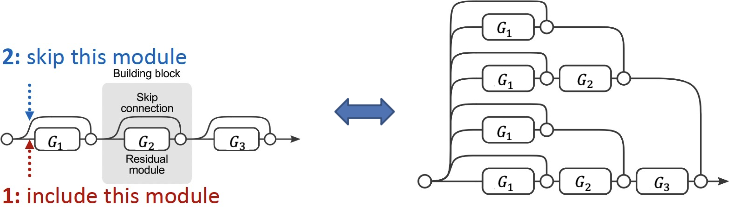
\includegraphics[height=0.025\textwidth]{figs/l6-7.png}
\hlorange{DropEdge }Randomly dropping some edges in the graph during each training epoch
\hlorange{PairNorm} Introduces a regularization term to force representations of nodes that are not connected to be different.
